\section{Command line interface} \label{sec:cli}
The StochBB installation comes with a command line tool. With this tool, a process definition
in XML (see Section \ref{sec:xml}) can be analyzed. The results are returned as CSV or they can be plotted
directly.

\subsection{Synopsis}
\begin{lstlisting}
 stochbb [OPTIONS] [CMD] INPUTFILE [OUTPUT OPTIONS]
\end{lstlisting}

\subsubsection{Options}
\begin{tabular}{p{.3\textwidth}p{.6\textwidth}}
 \code{--help} & Prints a short help string and exits. \\
 \code{--version} & Prints the version string and exits. \\
 \code{--log-debug} &Prints debug messages to stderr. By default, only warnings and error messages
  are printed to stderr. 
\end{tabular}

\subsubsection{Commands}
\begin{tabular}{p{.3\textwidth}p{.6\textwidth}}
 \code{pdf} & Specifies to evaluate the PDF of the variables selected in the \code{INPUTFILE} (default). \\
 \code{cdf} & Specifies to evaluate the CDF instead of the PDF of the variables selected in the
  \code{INPUTFILE}. \\
 \code{sample} & Samples from the variables selected in the \code{INPUTFILE}.
\end{tabular}

\subsubsection{Output options}
\begin{tabular}{p{.3\textwidth}p{.6\textwidth}}
 \code{--plot} & Plots the marginal PDFs or CDFs of the output variables specified in the \code{INPUTFILE}. \\
 \code{--csv=FILENAME} & Writes the PDFs or CDFs of the output variables specified in the \code{INPUTFILE}
  to \code{FILENAME}.
\end{tabular}

By default, the results (evaluated PDFs, CDFs or drawn samples) are printed to stdout, allowing for the direct usage 
of the results by other command line tools.

\subsection{Examples}
The following examples use the following system definition stored in a file name \code{example.xml}:
\begin{lstlisting}[language=XML]
<?xml version="1.0"?>

<simulation xmlns="http://hmatuschek.github.io/stochbb/simulation-0.0.dtd"
            xmlns:m="http://www.w3.org/1998/Math/MathML">

 <load>exp.xml</load>

 <var type="exp" id="X1">
  <param name="lambda"> <m:cn>0.01</m:cn> </param>
 </var>

 <var type="exp" id="X2">
  <param name="lambda"> <m:cn>0.02</m:cn> </param>
 </var>

 <var type="maximum" id="max" name="max(X1,X2)">
  <var ref="X1"/> <var ref="X2"/>
 </var>

 <output from="0" to="300" steps="1000">
  <var ref="X1"/> <var ref="X2"/> <var ref="max"/>
 </output>
</simulation>
\end{lstlisting}

Using this example system, the following call plots the PDFs of the random variables \code{X1}, \code{X2} and \code{max} defined in XML above
\begin{lstlisting}
 stochbb pdf example.xml --plot
\end{lstlisting}
The resulting plot is shown in Figure \ref{fig:exampleplot1}.	

\begin{figure}
 \centering
  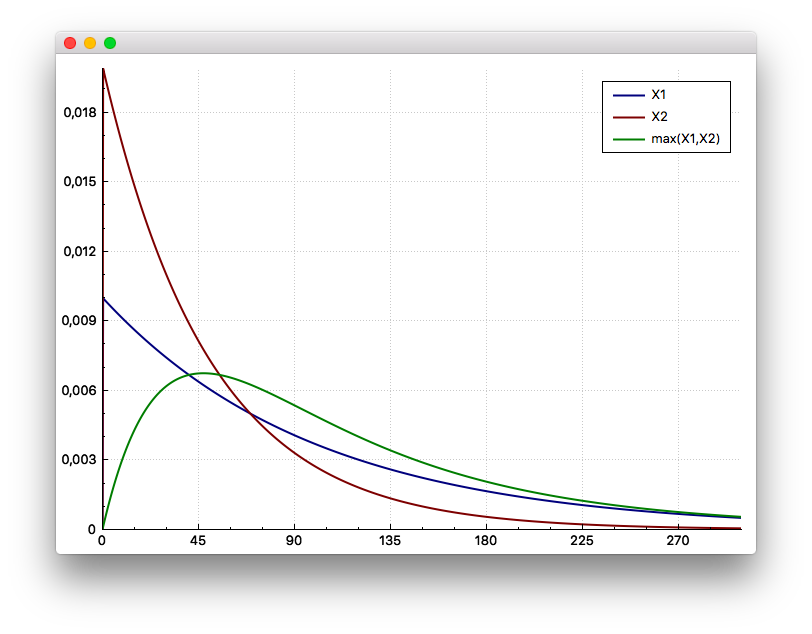
\includegraphics[width=0.7\textwidth]{exampleplot1.png}
  \caption{Plot of the marginal PDFs of the random variables $X_1\sim \text{Exp}(0.01)$, $X_2\sim \text{Exp}(0.02)$ and 
	$max = \max\{X_1,X_2\}$ as generated by the \code{stochbb} command line tool.} \label{fig:exampleplot1}
\end{figure}

The same PDF can be stored as CSV in \code{output.csv} by calling
\begin{lstlisting}
 stochbb pdf example.xml --csv=output.csv
\end{lstlisting}
or printed to stdout by calling 
\begin{lstlisting}
 sotchbb pdf example.xml
\end{lstlisting}

Finally, the call
\begin{lstlisting}
 sotchbb sample example.xml --csv=output.csv
\end{lstlisting}
draws 1000 samples of the random variables \code{X1}, \code{X2} and \code{max} defined in XML above.
